\documentclass[]{article}
\usepackage{lmodern}
\usepackage{amssymb,amsmath}
\usepackage{ifxetex,ifluatex}
\usepackage{fixltx2e} % provides \textsubscript
\ifnum 0\ifxetex 1\fi\ifluatex 1\fi=0 % if pdftex
  \usepackage[T1]{fontenc}
  \usepackage[utf8]{inputenc}
\else % if luatex or xelatex
  \ifxetex
    \usepackage{mathspec}
  \else
    \usepackage{fontspec}
  \fi
  \defaultfontfeatures{Ligatures=TeX,Scale=MatchLowercase}
\fi
% use upquote if available, for straight quotes in verbatim environments
\IfFileExists{upquote.sty}{\usepackage{upquote}}{}
% use microtype if available
\IfFileExists{microtype.sty}{%
\usepackage{microtype}
\UseMicrotypeSet[protrusion]{basicmath} % disable protrusion for tt fonts
}{}
\usepackage[margin=1in]{geometry}
\usepackage{hyperref}
\hypersetup{unicode=true,
            pdftitle={Supplementary Materials: A gene-diet interaction-based score predicts response to dietary fat in the Women's Health Initiative},
            pdfborder={0 0 0},
            breaklinks=true}
\urlstyle{same}  % don't use monospace font for urls
\usepackage{graphicx,grffile}
\makeatletter
\def\maxwidth{\ifdim\Gin@nat@width>\linewidth\linewidth\else\Gin@nat@width\fi}
\def\maxheight{\ifdim\Gin@nat@height>\textheight\textheight\else\Gin@nat@height\fi}
\makeatother
% Scale images if necessary, so that they will not overflow the page
% margins by default, and it is still possible to overwrite the defaults
% using explicit options in \includegraphics[width, height, ...]{}
\setkeys{Gin}{width=\maxwidth,height=\maxheight,keepaspectratio}
\IfFileExists{parskip.sty}{%
\usepackage{parskip}
}{% else
\setlength{\parindent}{0pt}
\setlength{\parskip}{6pt plus 2pt minus 1pt}
}
\setlength{\emergencystretch}{3em}  % prevent overfull lines
\providecommand{\tightlist}{%
  \setlength{\itemsep}{0pt}\setlength{\parskip}{0pt}}
\setcounter{secnumdepth}{0}
% Redefines (sub)paragraphs to behave more like sections
\ifx\paragraph\undefined\else
\let\oldparagraph\paragraph
\renewcommand{\paragraph}[1]{\oldparagraph{#1}\mbox{}}
\fi
\ifx\subparagraph\undefined\else
\let\oldsubparagraph\subparagraph
\renewcommand{\subparagraph}[1]{\oldsubparagraph{#1}\mbox{}}
\fi

%%% Use protect on footnotes to avoid problems with footnotes in titles
\let\rmarkdownfootnote\footnote%
\def\footnote{\protect\rmarkdownfootnote}

%%% Change title format to be more compact
\usepackage{titling}

% Create subtitle command for use in maketitle
\providecommand{\subtitle}[1]{
  \posttitle{
    \begin{center}\large#1\end{center}
    }
}

\setlength{\droptitle}{-2em}

  \title{Supplementary Materials: A gene-diet interaction-based score predicts
response to dietary fat in the Women's Health Initiative}
    \pretitle{\vspace{\droptitle}\centering\huge}
  \posttitle{\par}
    \author{}
    \preauthor{}\postauthor{}
    \date{}
    \predate{}\postdate{}
  
\usepackage{booktabs}
\usepackage{longtable}
\usepackage{array}
\usepackage{multirow}
\usepackage{wrapfig}
\usepackage{float}
\usepackage{colortbl}
\usepackage{pdflscape}
\usepackage{tabu}
\usepackage{threeparttable}
\usepackage{threeparttablex}
\usepackage[normalem]{ulem}
\usepackage{makecell}
\usepackage{xcolor}

\begin{document}
\maketitle

\newcommand{\beginsupplement}{%
        \setcounter{table}{0}
        \renewcommand{\thetable}{S\arabic{table}}%
        \setcounter{figure}{0}
        \renewcommand{\thefigure}{S\arabic{figure}}%
     }
%
        \setcounter{table}{0}
        \renewcommand{\thetable}{S\arabic{table}}%
        \setcounter{figure}{0}
        \renewcommand{\thefigure}{S\arabic{figure}}%

\begin{ThreePartTable}
\begin{TableNotes}
\item Power calculations were undertaken using the Quanto tool, with parameters set as follows: additive model, SNP main effect of 0.5\% of trait variance, binary environment with 50\% prevalence, and environmental effect explaining 10\% of the trait variance.
\end{TableNotes}
\begin{longtable}{rrrr}
\caption{\label{tab:show-power-calcs}Sample size necessary to achieve power of 0.8}\\
\toprule
GxE variance explained (\%) & N (nominal) & N (suggestive) & N (genome-wide)\\
\midrule
0.05 & 14046 & 49488 & 70866\\
0.10 & 7021 & 24737 & 35423\\
0.50 & 1401 & 4936 & 7069\\
1.00 & 699 & 2461 & 3524\\
\bottomrule
\insertTableNotes
\end{longtable}
\end{ThreePartTable}

\begin{figure}
\centering
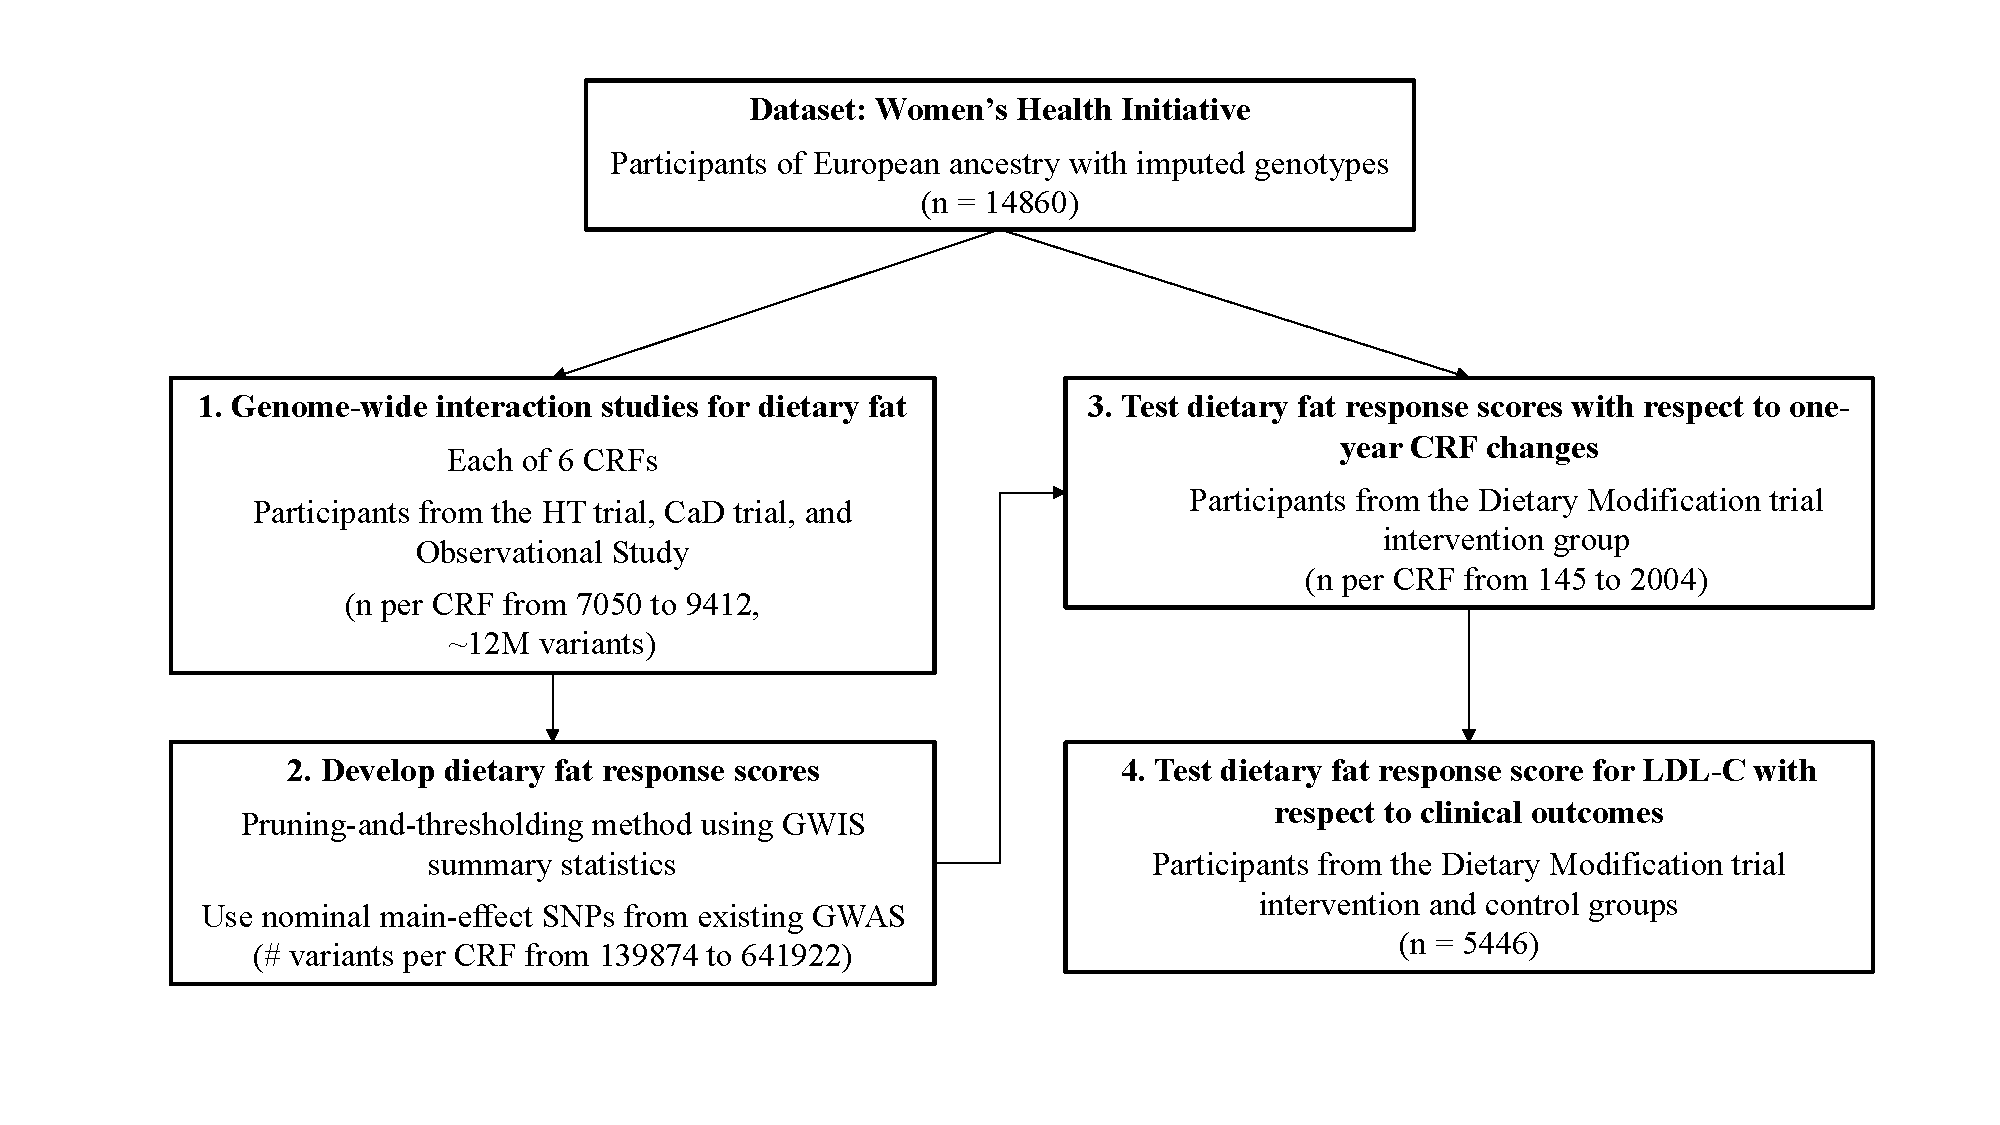
\includegraphics{workflow.pdf}
\caption{Workflow of the study. First, a series of genome-wide
interaction studies (GWIS) were conducted with dietary fat as the
exposure for each of six cardiovascular risk factors (CRFs). Next,
dietary fat response scores were developed using GWIS summary statistics
and tested for the prediction of one-year CRF changes in the Dietary
Modification trial intervention arm. Finally, the LDL-C score was tested
for the prediction of differential effects on chronic disease
development over approximately twenty years of follow-up.}
\end{figure}

\begin{figure}
\centering
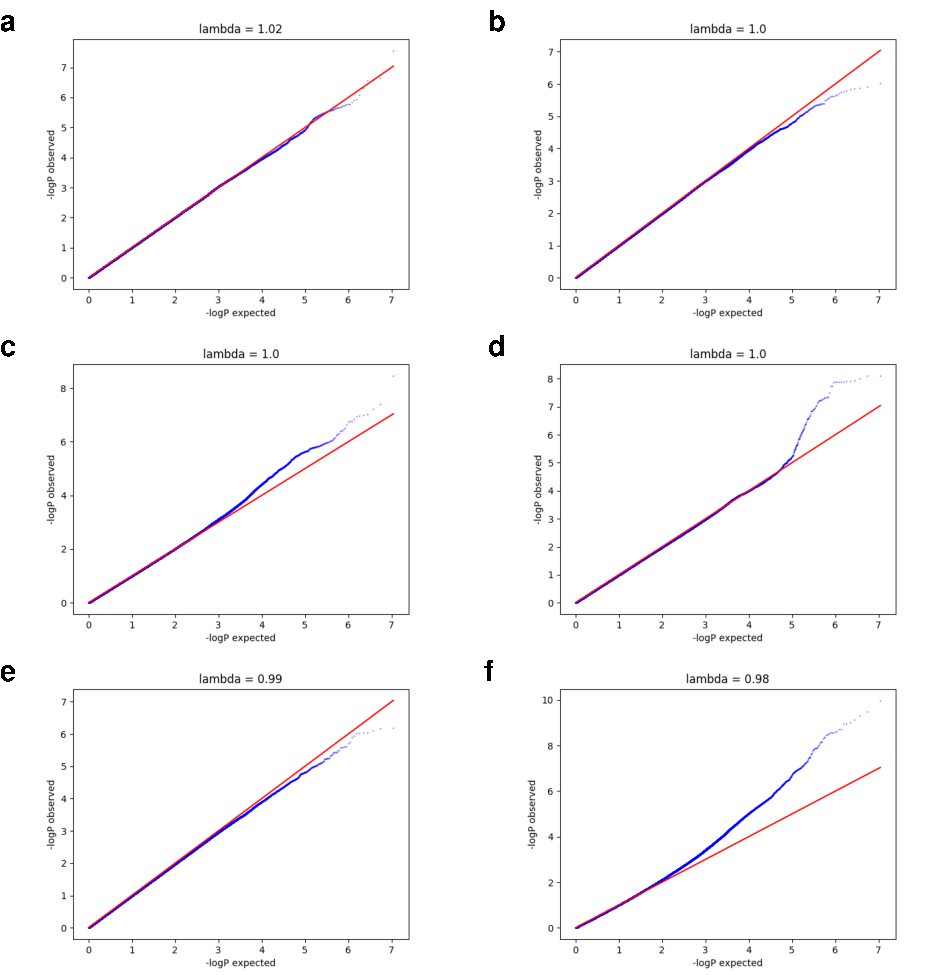
\includegraphics{figures/show-qq-plots-1.pdf}
\caption{Q-Q plots from individual CRF GWIS. The distribution of
p-values from each GWIS is plotted against the expected uniform p-value
distribution. Plots correspond to: a) BMI, b) SBP, c) LDL-C, d) HDL-C,
e) TG, and f) FG.}
\end{figure}

\begin{ThreePartTable}
\begin{TableNotes}
\item[1] Sample size available with 1-year follow-up for each CRF
\item[2] Number of SNPs selected by the pruning-and-thresholding algorithm for each CRF-threshold combination
\item[3] Standardized effect size (SES) represents the regression coefficient estimate in terms of CRF standard deviation per responder score standard deviation
\end{TableNotes}
\begin{longtable}{lllllllllll}
\caption{\label{tab:show-test-scores-alternate-filters}Responder score effects on CRF changes in DM trial participants across main-effect filter thresholds}\\
\toprule
\multicolumn{2}{c}{ } & \multicolumn{3}{c}{All variants} & \multicolumn{3}{c}{Nominal main effect (p<0.05)} & \multicolumn{3}{c}{Suggestive main effect (p<1e-5)} \\
\cmidrule(l{3pt}r{3pt}){3-5} \cmidrule(l{3pt}r{3pt}){6-8} \cmidrule(l{3pt}r{3pt}){9-11}
CRF & N\textsuperscript{1} & \# SNPs\textsuperscript{2} & SES\textsuperscript{3} & P-value & \# SNPs\textsuperscript{2} & SES\textsuperscript{3} & P-value & \# SNPs\textsuperscript{2} & SES\textsuperscript{3} & P-value\\
\midrule
BMI & 1988 & 158365 & 0.049 & 0.026 & 6042 & 0.027 & 0.221 & 569 & 0.027 & 0.236\\
FG & 281 & 161906 & -0.078 & 0.495 & 1924 & 0.016 & 0.791 & 7 & 0.006 & 0.92\\
HDL-C & 150 & 153942 & 0.028 & 0.63 & 1731 & -0.06 & 0.471 & 42 & 0.085 & 0.258\\
LDL-C & 145 & 156313 & 0.035 & 0.729 & 1760 & -0.179 & 0.026 & 46 & 0.01 & 0.901\\
SBP & 2004 & 153942 & -0.016 & 0.473 & 1536 & 0.029 & 0.196 & 6 & 0 & 0.999\\
TG & 150 & 152006 & -0.184 & 0.203 & 1774 & -0.139 & 0.066 & 47 & -0.043 & 0.573\\
\bottomrule
\insertTableNotes
\end{longtable}
\end{ThreePartTable}

\begin{ThreePartTable}
\begin{TableNotes}
\item[1] Standardized effect size (SES) represents the regression coefficient estimate in terms of CRF standard deviation per responder score standard deviation
\end{TableNotes}
\begin{longtable}{llllllllll}
\caption{\label{tab:show-test-scores-cross-ancestry}Responder score effects on CRF changes in DM trial participants across ancestries}\\
\toprule
\multicolumn{1}{c}{} & \multicolumn{3}{c}{All combined} & \multicolumn{3}{c}{Black} & \multicolumn{3}{c}{Hispanic} \\
\cmidrule(l{3pt}r{3pt}){2-4} \cmidrule(l{3pt}r{3pt}){5-7} \cmidrule(l{3pt}r{3pt}){8-10}
CRF & N & SES\textsuperscript{1} & P-value & N & SES\textsuperscript{1} & P-value & N & SES\textsuperscript{1} & P-value\\
\midrule
BMI & 3606 & -0.02 & 0.24 & 1214 & 0 & 0.994 & 404 & 0.018 & 0.719\\
FG & 572 & 0.08 & 0.043 & 214 & -0.004 & 0.955 & 77 & -0.014 & 0.901\\
HDL-C & 430 & -0.06 & 0.224 & 206 & -0.096 & 0.182 & 74 & -0.057 & 0.66\\
LDL-C & 422 & 0.084 & 0.066 & 206 & 0.055 & 0.412 & 71 & 0.126 & 0.227\\
SBP & 3645 & 0.041 & 0.015 & 1230 & 0 & 0.991 & 411 & -0.008 & 0.868\\
TG & 430 & -0.075 & 0.112 & 206 & -0.023 & 0.743 & 74 & -0.098 & 0.433\\
\bottomrule
\insertTableNotes
\end{longtable}
\end{ThreePartTable}

\begin{ThreePartTable}
\begin{TableNotes}
\item[1] Std. effect size represents the regression coefficient estimate in terms of CRF standard deviation per responder score standard deviation
\end{TableNotes}
\begin{longtable}{lrrrr}
\caption{\label{tab:show-test-ldl-scores-other-rfs}LDL-FRS effects on alternate CRF changes in DM trial participants}\\
\toprule
Outcome risk factor & \# SNPs in risk score & Sample size & Std. effect size\textsuperscript{1} & P-value\\
\midrule
BMI & 1747 & 1988 & -0.02 & 0.36\\
SBP & 1747 & 2004 & 0.00 & 0.83\\
HDL-C & 1747 & 150 & -0.07 & 0.39\\
TG & 1747 & 150 & 0.11 & 0.16\\
FG & 1747 & 281 & 0.01 & 0.82\\
\bottomrule
\insertTableNotes
\end{longtable}
\end{ThreePartTable}


\end{document}
